\chapter{テトリスのブロックを作る}
この章からはプログラムの例を示しません。今までのファイルに追記していく形になります。
\section{ブロックの設計}
\subsection{ブロックの機能を考える}
ブロックは、テトリスの中心的な要素です。ブロックはどんな機能を持つといいでしょうか?
\subsubsection{ブロックの機能}
\begin{itemize}
  \item ブロックを回転させる関数
  \item ブロックを指定した位置に描画する関数
\end{itemize}

\section{ブロックの表示方法を考える}
\subsection{設計}
今回の設計では描画する関数はBoardに任せられています。
しかし、Boardはどんな形のブロックを書くのかわからないのでどうにかしてブロックの情報を
やり取りする必要があります。よって、設計する際にはブロックのクラス、Boardのクラス
両方に機能を加えます。
\subsubsection{設計の案}
\begin{itemize}
  \item Boardが現在保持中のブロックの変数を持つ
  \item Boardはその変数に情報を要求して、その変数は塗らなければいけないマスの座標をリストで返す。これをblock\_info関数とする。
  \item Boardはそのリストをもとに、drawの途中で画面に書き込むことにする
\end{itemize}

図にするとこんな感じです。
\begin{figure}[h]
  \centering
  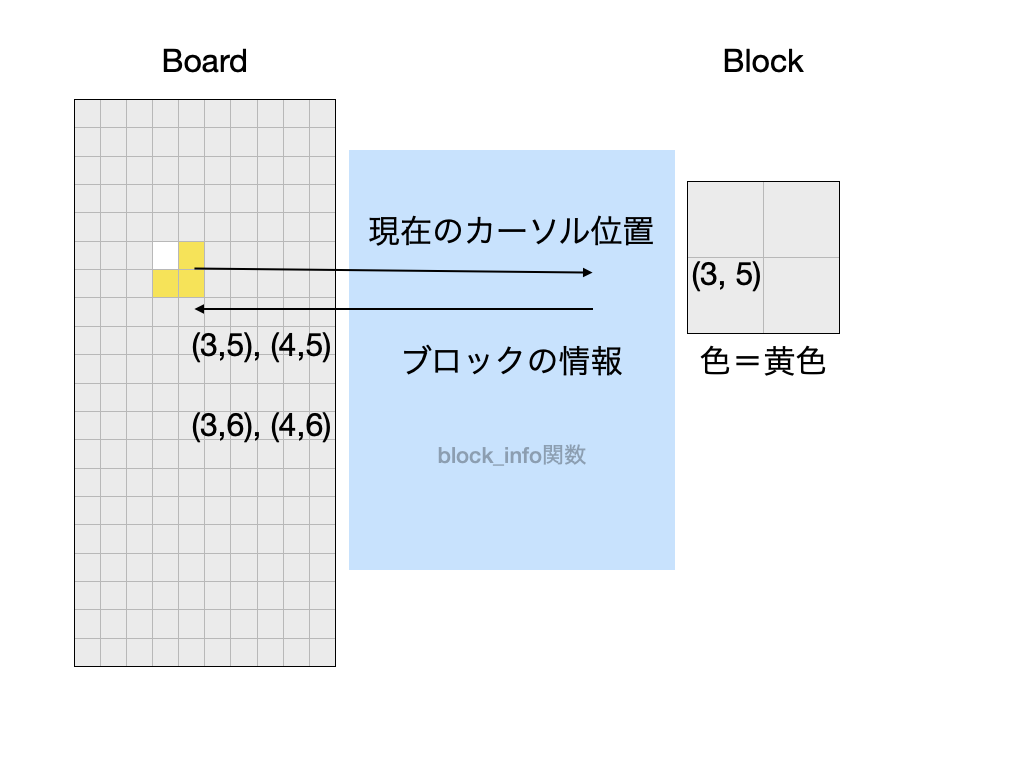
\includegraphics[width=100mm]{images/BoardAndBlock.png}
  \caption{BoardとBlockのやりとり}
\end{figure}

Boardが現在保持中のブロックの変数を持つということなので、Boardクラスに変数を追加します。
最初は何も持っていないので、「動いているブロック」という意味の「moving\_block」にPythonの特別な空を表す「None」を入れておきます。
さらに、ブロックの描画を行う処理をBoardクラスに追加します。画面に書く処理はdraw関数でしたね。
draw関数は現在の盤面を塗る(動かしているブロックは対象外)→カーソルを描く→グリッドを描く、という順番で行われていました。
どこに動かしているブロックを描く処理を入れるか考えてみましょう。
\lstinputlisting[caption={Boardクラスの変更点}, language=Python]{chapter6/ch6_2_1.py}
\texttt{"""..."""}は自分で書いてみましょう。変数の名前を変にしすぎると
先生が助けにくくなります。

\section{ブロックのクラスを定義する}
\subsection{OBlockクラスを定義する}
今回はOブロックを作ります。Oブロックは一番簡単なブロックです。2x2の黄色の正方形です。
最初にこれから作ることにしたのは、回転が必要ないからです。
ブロックにはどのような機能が必要だったか思い出してみます。
\begin{itemize}
  \item ブロックを回転させる関数
  \item 自分の色をもつ変数
  \item ブロックの情報を返す関数
\end{itemize}
\newpage
\lstinputlisting[caption=OBlockクラスの作成, language=Python]{chapter6/ch6_2_2.py}
block\_info関数はカーソルの位置を受け取って、
そこからカーソルの位置、右、下、右下の4つのマスを返します。
Boardはその座標とOBlockの中にあるcolor変数を使って描画します。
rotate関数は今回は作っていませんが、ブロックの種類によっては必要になります。

\section{ブロックを表示させてみる}
\subsection{main関数を変更する}
main関数を変更して、OBlockを動かしてみましょう。
\lstinputlisting[caption={OBlockのテスト}, language=Python]{chapter6/ch6_3_1.py}
うまくいっていれば、Oブロックが動くはずです。
\newpage
\begin{figure}[h]
  \centering
  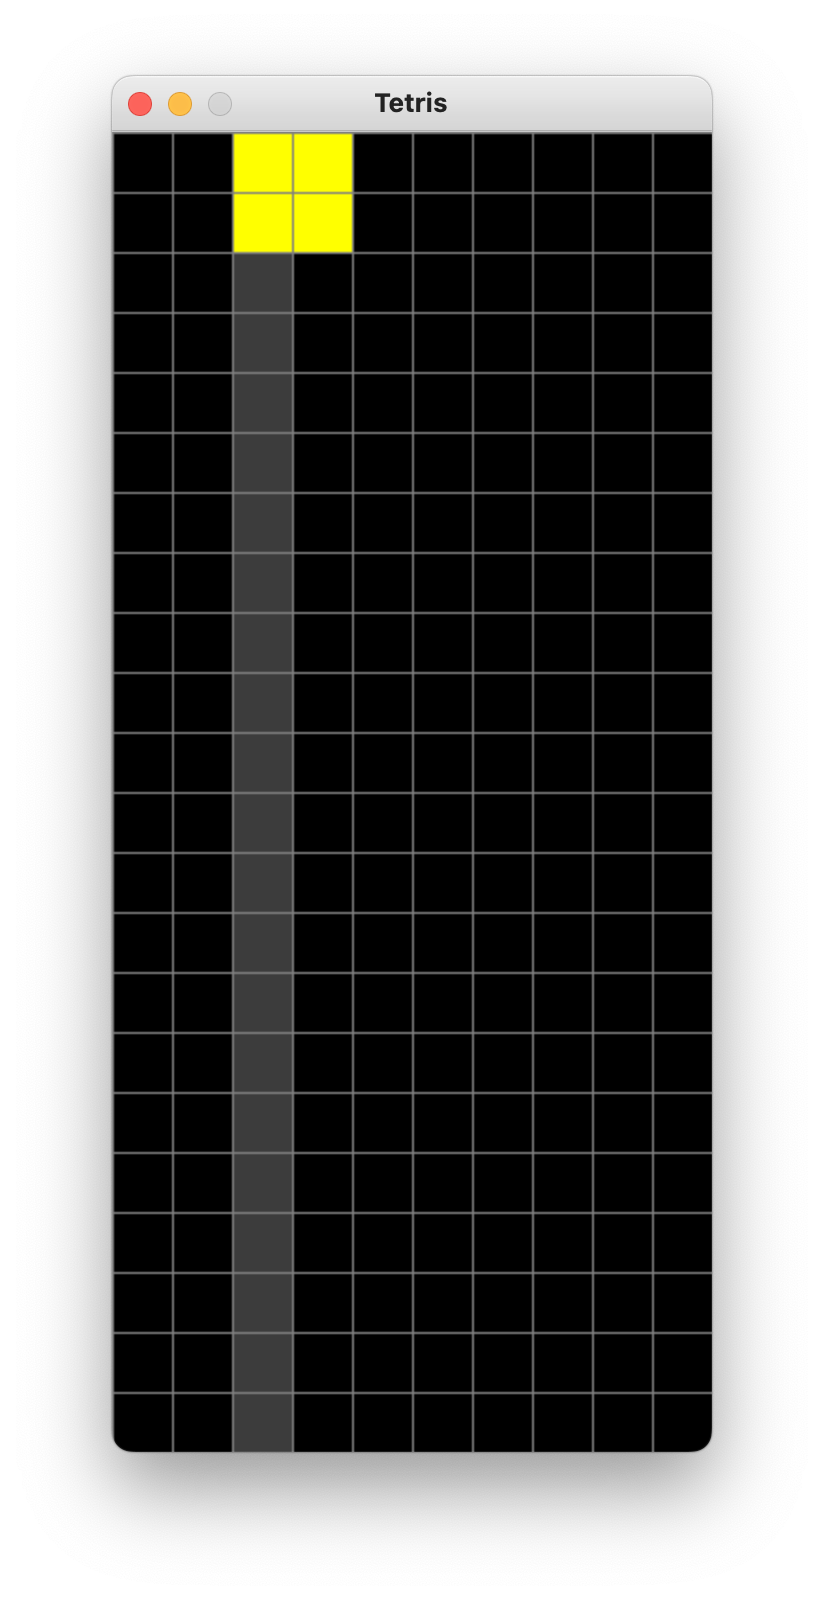
\includegraphics[height=80mm]{images/TetrisCH7.png}
  \caption{テトリスの実行結果}
\end{figure}
\newpage
ここで右端に動いてみましょう。ブロックが半分消えてしまいますね。

\subsection{ブロックの移動範囲を制限する}
この問題を解決するために、ブロックの移動範囲を制限する機能を追加します。
キー入力を受け取ってから動くまでの間に、ブロックが動けるかどうかを判定する処理を入れます。
さて、どこに入れるといいでしょうか?
\subsubsection{設計}
\begin{itemize}
  \item main関数が判定する
  \item Boardが判定する
  \item Cursorが判定する
  \item OBlockが判定する
\end{itemize}
クラスを使う前まではmain関数が判定するのが一般的でした。
しかし、今回はmainには余計な仕事をさせないようにしましょう。
動きを担当するのはCursorの役割です。Cursorにmove\_right関数などを
追加していたはずです。ここを次のように変更することで対処します。
\begin{itemize}
  \item OBlockはCursor, Boardから動けるかどうか計算する
  \item Cursorはその情報をもとに動くかどうか決める
\end{itemize}

\subsection{OBlockクラスを変更する}
OBlockクラスに、動ける範囲を計算する関数を追加します。
\lstinputlisting[caption={OBlockクラスの変更}, language=Python]{chapter6/ch6_3_2.py}
さて、次にカーソルの動きを変更します。
今までは無条件に動いていましたが、一度ブロックを受け取って動けるか
どうかを判定してもらい、動けるなら動くようにします。

\subsection{Cursorクラスを変更する}
\lstinputlisting[caption={Cursorクラスの変更}, language=Python]{chapter6/ch6_3_3.py}
これらの変更が終わると、main.pyにエラーが出ているはずです。
今まではcursor.move\_right()のように書いていましたが、
これからは引数としてboardとblockを渡す必要があるからです。
もちろん、main関数で引数を渡すように変更しても良いのですが、
少し見栄えが悪いので(プログラマとしては見栄えが悪いです)、変更を加えます。
\subsection{Boardクラスを変更する}
今回はカプセル化という方法で、BoardクラスがCursorをカプセルのように閉じ込めて、
Board経由でCursorを操作するようにします。
そこで、Boardクラスにmove\_right関数を追加し、Cursorのmove\_right関数を呼び出すようにします。
\lstinputlisting[caption={Boardクラスの変更}, language=Python]{chapter6/ch6_3_4.py}
\subsection{main関数の変更}
最後に、main関数を変更して、cursorを使うのではなく、boardの移動機能を使うようにします。
\lstinputlisting[caption={main関数の変更}, language=Python]{chapter6/ch6_3_5.py}
これを実行すると、ブロックが右端に行かなくなります。
また、下方向にも消えずに止まるようになります。

\section{まとめ}
今回は、簡単なOBlockを作成しました。Boardクラスにブロックの情報を持たせ、
Boardは適宜OBlockに情報を要求して描画するようにしました。
また、ブロックの移動範囲を制限する機能を追加し、Cursorクラスにその機能を持たせました。
最後に、main関数を変更して、CursorではなくBoardを使ってブロックを動かすようにしました。

\subsubsection{懺悔}
正直にいうとこのテトリスの設計、若干失敗したなあと思っています。
今はBoardがmoving\_blockを持っています。しかし今回の章でいえば、ブロックをCursorの中に持たせるべきでした。
そうであればBoardがCursorをカプセル化する必要もなかった上に設計が簡単になります。
今後ブロックを落とす処理を追加するときを見越してこのような設計にしたのでいいのですが、
果たしてこれが正解だったのか、今後の展開にご期待ください。